49. \begin{figure}[ht!]
\center{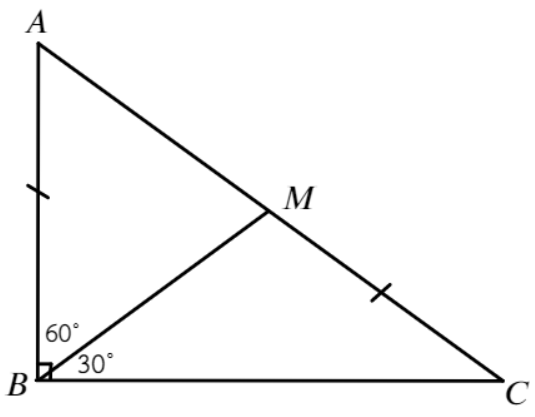
\includegraphics[scale=0.35]{g9-49.png}}
\end{figure}\\
Из теорем синусов для треугольников $AMB$ и $CMB$ получим равенства\\ $\cfrac{AB}{\sin(AMB)}=\cfrac{AM}{\sin(60^\circ)},\ \cfrac{BC}{\sin(\angle BMC)}= \cfrac{MC}{\sin(30^\circ)}.$ Так как синусы смежных углов равны, после деления равенств друг на друга получим соотношение $\cfrac{AB}{BC}=\cfrac{AM\cdot\cfrac{1}{2}}{MC\cdot\cfrac{\sqrt{3}}{2}},$ откуда $AM\cdot BC=4\sqrt{3}.$ Пусть $BC=x,$ тогда $AM=\cfrac{4\sqrt{3}}{x}.$ По теореме Пифагора имеем $x^2+4=\left(\cfrac{4\sqrt{3}}{x}+2
ight)^2,\ x^2+4=\cfrac{48}{x^2}+\cfrac{16\sqrt{3}}{x}+4,\ x^4-16\sqrt{3}x-48=0,\ x^4-2\sqrt{3}x^3+2\sqrt{3}x^3-12x^2+12x^2-24\sqrt{3}x+8\sqrt{3}x-48=0,$\\
$x^3(x-2\sqrt{3})+2\sqrt{3}x^2(x-2\sqrt{3})+12x(x-2\sqrt{3})+8\sqrt{3}(x-2\sqrt{3})=0,\ (x-2\sqrt{3})(x^3+2\sqrt{3}x^2+12x+8\sqrt{3})=0,\ x=2\sqrt{3}$см. Решение единственно, так как $x>0.$\\
